%%% ===============chapter 6 starts here ============================

\chapter{Conclusion}\label{ch:conclusion}

\section{Contribution to Research and Literature} My contribution would be included in this section.

\section{Recent Developments in Chapter \ref{ch:largepsmalln}}

In some situations where the number of dimensions ($p$) is approximately equal or close to the number of observations ($n$), we may see separation among the groups when a linear discriminant analysis (LDA) or a penalized discriminant analysis (PDA) is performed. A natural question is whether there is actually a real separation among the groups or we observed the separation due to the fact that $p \approx n$ or $p > n$. Let us consider the following example of LDA method used to classify the groups of paper wasps. There are 50 different paper wasps divided into 4 groups: Foundress (F), Gyne (G), Queen (Q) and Worker (W). There are 14 paper wasps of type Foundress and 12 each of the other 3 types. The authors, knowing that LDA requires that the number of observations ($n$) should be larger than ($p$), randomly selected a subset of 40 significantly different oligonucleotides from a total of 447 oligonucleotides. Figure \ref{oligo} shows the scatterplot of LD1 versus LD2.

\begin{figure*}[hbtp]
%\begin{figurehere}
   \centering
       \scalebox{.50}{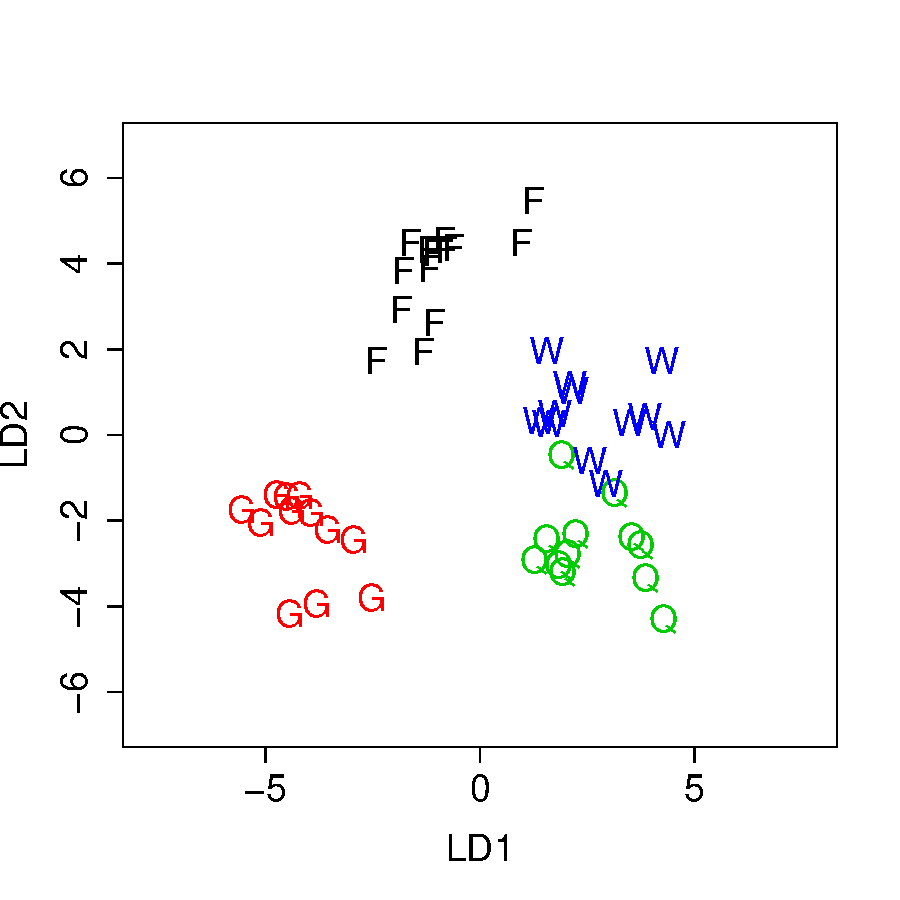
\includegraphics{toth_lda.pdf}}
       \caption{LD1 versus LD2 from an LDA on a randomly selected subset of 40 significantly different oligos. F, Foundress; G, gyne; Q, queen and W, worker.}
     \label{oligo}
%\end{figurehere}
\end{figure*}  

Figure \ref{oligo} clearly shows that groups Foundress(F) and Gyne(G) are two separated clusters while the groups Worker(W) and Queen(Q) are not separated and forms a separate cluster. It would be interesting to find whether the separation is real.

We obtained the wasp data used to generate Figure \ref{oligo} from the authors. To check whether the separation is real, we generate a lineup by using the wasp data as the actual data. We generate the lineup by randomly permuting the group variable and breaking any relationship between the variables  and the group. Figure \ref{toth_lineup} shows the lineup plots of LD1 versus LD2 of a LDA of the 40 randomly selected oligos.

\begin{figure*}[hbtp]
%\begin{figurehere}
   \centering
       \scalebox{1}{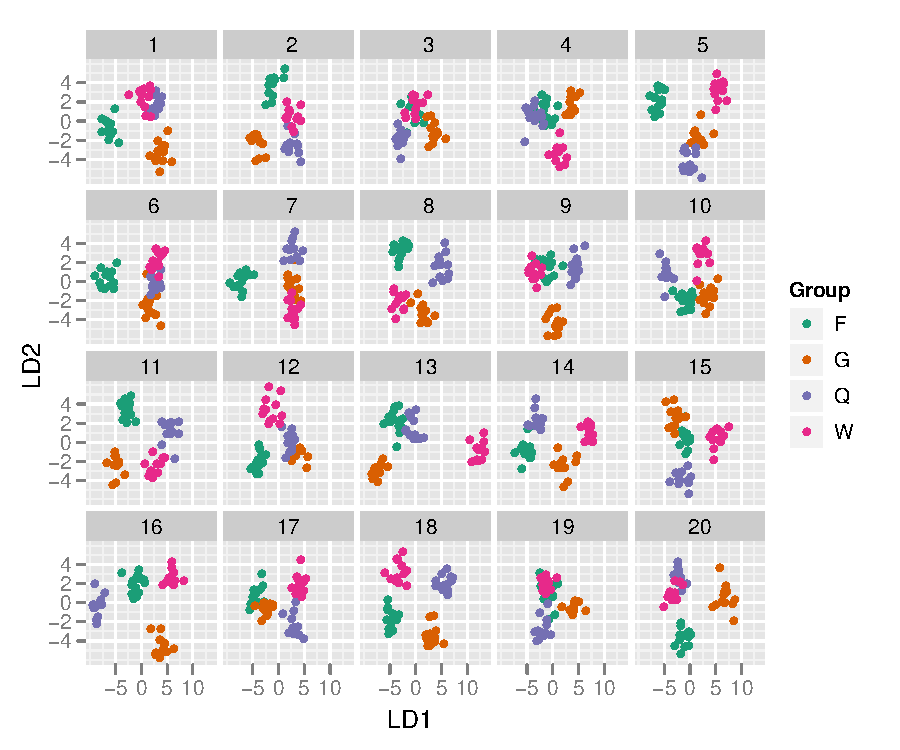
\includegraphics{toth_lineup_lda.pdf}}
       \caption{Lineup Plot showing LD1 versus LD2 from an LDA on a randomly selected subset of 40 significantly different oligos. F, Foundress; G, gyne; Q, queen and W, worker. The actual data plot is placed randomly among 19 null plots. Can you identify the actual data?  }
       \label{toth_lineup}
\end{figure*} 

In Figure \ref{toth_lineup} we can see that the clusters are separated even after breaking any dependency between the groups and the variables. Since PDA is a better index than LDA in a large $p$ situation, we used PDA to generate another lineup which is presented in Figure \ref{toth_pda}. In Figure \ref{toth_pda}, the clusters are not even separated and we cannot identify the true plot. We also generated 40 dimensions of random noise with 50 observations in each dimension. A group variable is also added as the one present in the wasp data. We performed a LDA on this random noise data and we can can still see clusters.  This shows that the separation seen in Figure \ref{oligo} may not be real but appear only due to the fact that the number of variables are large.

\begin{figure*}[hbtp]
%\begin{figurehere}
   \centering
       \scalebox{1}{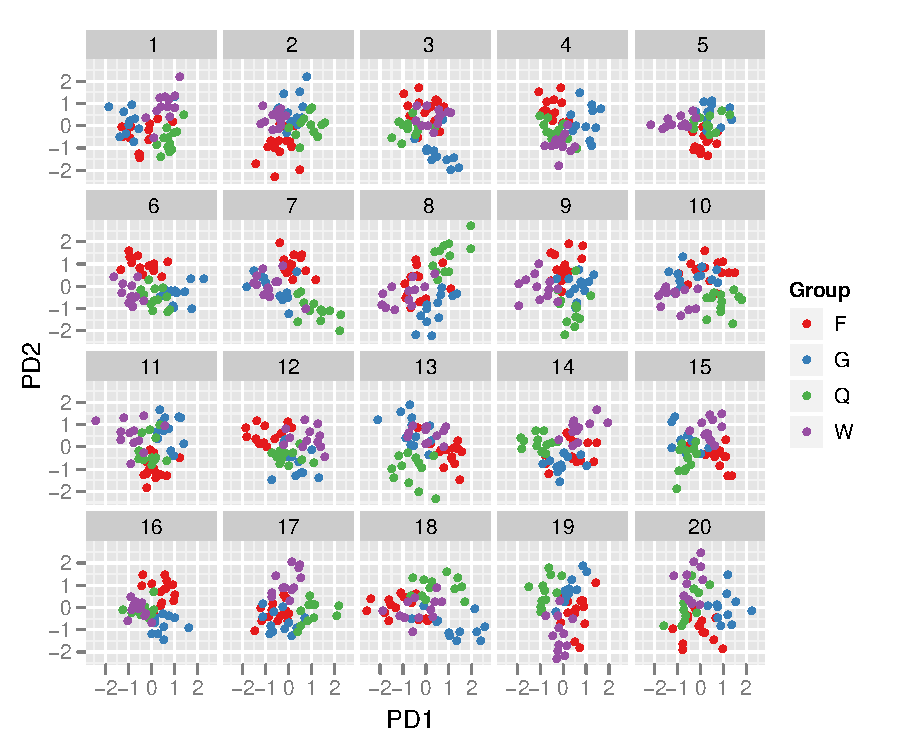
\includegraphics{toth_lineup_pda.pdf}}
       \caption{Lineup Plot showing PD1 versus PD2 from an PDA on a randomly selected subset of 40 significantly different oligos. F, Foundress; G, gyne; Q, queen and W, worker. The actual data plot is placed randomly among 19 null plots. Can you identify the actual data?  }
       \label{toth_pda}
\end{figure*}   


\section{Recent Developments in Chapter \ref{ch:waldo}}

\section{Distance measures}

We looked at some of the other distance measures. Our goal now is to find a distance measure which best represents the visual distance.

\begin{itemize}


\item Euclidean Distance of permutations: The Euclidean distance of permutations $P$ is 
\[
d^2_P(X) = \sum_{i=1}^n ( i - P(i))^2.
\]
where $i = \{1, 2, ..., n\}$


\item Canberra Distance: Using exactly the same setup as the binned distance , the canberra distance under permutation is defined as
%\begin{eqnarray*}
\[
c^2_P(X)  = \left \{ 
\begin{array}{ll}
\sum_{i=1}^p \sum_{j=1}^q \frac{ |C_{X_i,Y_j} - C_{X_i,P(Y)_j}|}{ C_{X_i,Y_j} + C_{X_i,P(Y)_j}} & \text{if } C_{X_i,Y_j} + C_{X_i,P(Y)_j} > 0,\\
0 & \text{otherwise},
\end{array} \right.
\]
Like the binned distance, the canberra distance is also effected by the number of bins used. Here again we use the usual convention as the binned distance. Canberra distance is an improvement to the binned distance as it puts less weight on the bins which has a large number of points than the bins with fewer points. Visually it is difficult to differentiate between a single point and a number of points having the exact coordinates. Canberra distance has the same drawbacks as the binned distance. So we defined the weighted canberra distance which is a similar measure as the weighted bin distance.

\item Weighted Canberra Distance:  Using the same setup of the weighted bin distance, the weighted canberra distance under permutation is defined as 
%\begin{eqnarray*}
\[
wc_P^2(X) = \left \{ 
\begin{array}{ll}
\sum_{i=1}^p \sum_{j=1}^q \frac{ |W_{X_i,Y_j} - W_{X_i,P(Y)_j}|}{ W_{X_i,Y_j} + W_{X_i,P(Y)_j}} & \text{if } W_{X_i,Y_j} + W_{X_i,P(Y)_j} > 0,\\
0 & \text{otherwise},
\end{array} \right.
\] 
%\end{eqnarray*}
where like the weighted bin distance, $W_{X_i,Y_i}$ denotes the joint (empirical) density of $X$, $Y$ at location $(X_i, Y_i)$. 

\item Correlation between $X$ and $[P]X$: Let $X$ be a continuous variable. The correlation between the $X$ and $[P]X$ is defined as
\[
r_P(X) = \frac{ \sum_{i=1}^n (X_i - \bar{X_i})(X_{P(i)} - \bar{X}_{P(i)})}{\sqrt{\sum_{i=1}^n (X_i - \bar{X_i})^2}\sqrt{\sum_{i=1}^n (X_{P(i)}- \bar{X}_{P(i)})^2}}.
\]

\item Hausdorff distance: Let $a \in A$ and $b \in B$ be two sets of points. The Hausdorff distance between A and B is defined as
 \[
H_P(X)  = max (h(A, B), h(B, A))
\]
where 
\begin{eqnarray*}
h(A, B) &:=& \max_{a \in A} \min_{b \in B} ||a - b|| \\ & = & \max_{a \in A} \min_{b \in B} \sqrt{\sum_{i=1}^n (a_i - b_i)^2}
\end{eqnarray*}
In our case $A$ and $B$ are the points whose coordinates are $(X_i, Y_i)$ and $(X_{P(i)}, Y_i)$ respectively. This measure is computationally intensive.

\end{itemize}


\section{Comparison of the distance measures}

For a particular dataset containing two continuous variables $X$ and $Y$, we generate 50 random datasets by permuting the $X$ variable but keeping the $Y$ variable fixed. We compute the distances between the actual data and each of the 50 permuted datasets by using all of the eleven distance measures defined above. We then plot a scatterplot matrix of the eleven distance measures. Figure \ref{scamat} gives the scatterplot matrix of the eleven distance measures.

\begin{figure}[htbp]
%\begin{figurehere}
   \centering
       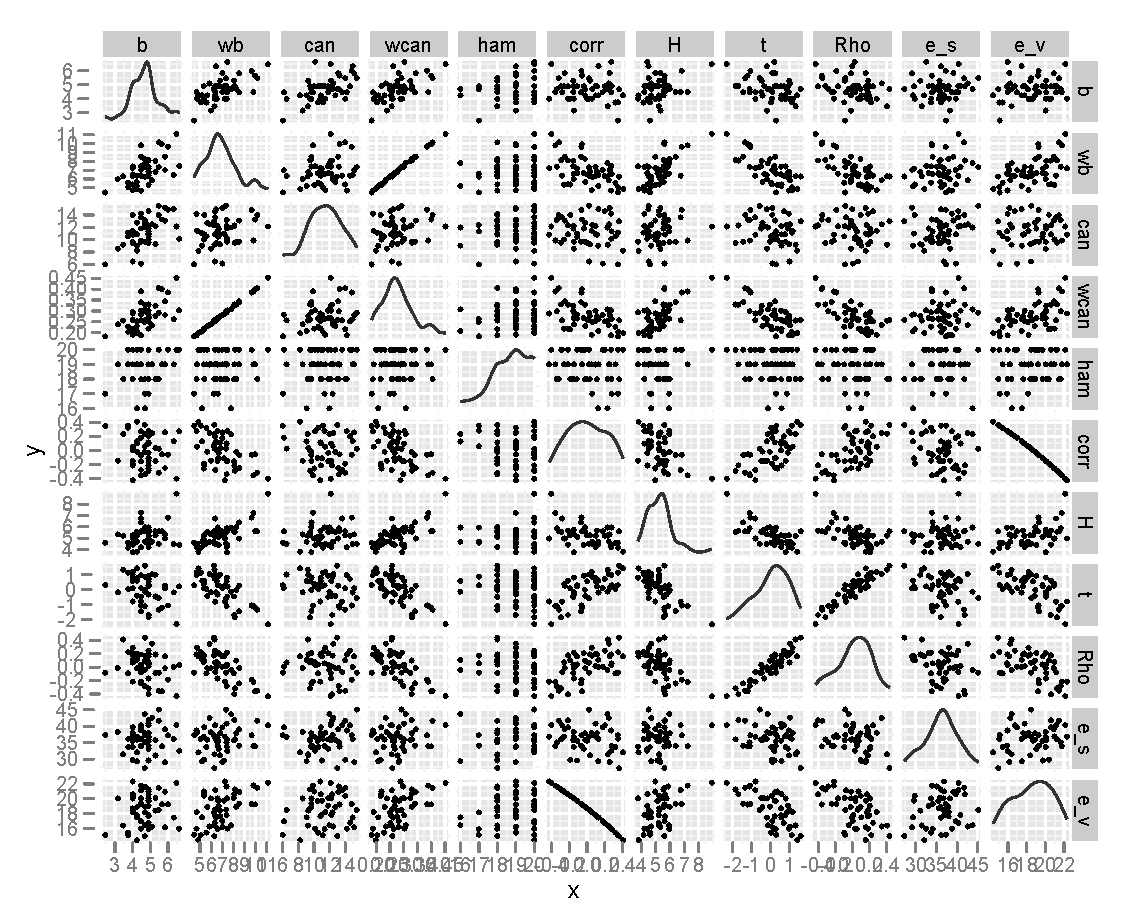
\includegraphics[width=5in]{sca_plot_matrix.pdf}
	\vspace{-.2in}
       \caption{Scatterplot matrix of the distance measures based on the 50 randomly generated datasets obtained by permuting the $X$ variable randomly 50 times.}
       \label{scamat}
\end{figure}

Figure \ref{scamat} shows that some of the distance measures are highly correlated, positive or negative. The weighted bin distance $w_P(X)$ is highly positively correlated to the weighted canberra distance $wc_P(X)$ and the correlation between $X$ and permuted $X$ ($r_P$) has a high negative correlation to the euclidean distance of the actual values ($d_V$). Also there is a fairly high correlation between t-statistic $t$ and Spearman's rank correlation $\rho$.  So it does not make sense to use all the distance measures as they do not explain the data differently. So we decided to exclude weighted canberra distance, euclidean distance of the actual values and Spearman's rank correlation $\rho$ from the analysis. So we have eight different measures.

\section{Visual Distance}

The main purpose is to find a distance measure from the eight shortlisted distance measures which describes the visual distance in the best possible way. Describing plots numerically with the help of a distance measure is next to impossible. But we want to find the distance measure which works in most situations in most types of data. \\

We are interested in datasets with two continuous variables. Let us assume $X$ and $Y$ are the two variables.  We permute one of the continuous variables, say $X$ by keeping the other variable (say $Y$) fixed to obtain one set of permuted data. We repeat the above process 10,000 times to obtain 10,000 randomly generated datasets. \\

We calculate the distance between the actual dataset and each of the 10,000 permuted datasets by using the eight shortlisted distance measures from the eleven defined in Section \ref{defn.distance}. Hence we have 10,000 of each of the distance measures. We select those permuted datasets which has the minimum distance from the actual dataset according to the eight distance measures. So we obtain eight permuted datasets which are the closest to the actual dataset. \\

The drawbacks with this procedure is that the hamming distance ($h_P$)  and the binned distance ($b_P$) have discrete distributions. Hence, according to these distance measures, in most situations there may be more than one dataset which have the minimum distance from the actual dataset. But we select any one of the datasets randomly. Also in some cases two or more distance measures may yield the same dataset as the one ``closest'' to the actual dataset. In these cases, we randomly select the other datasets from the 10,000 permuted datasets.   \\

Then we form a lineup with 3 rows and 3 columns by putting the actual dataset in the middle and randomly placing the other datasets in the other eight positions. Figure \ref{minimum} shows such a lineup.

\begin{figure}[htbp]
%\begin{figurehere}
   \centering
       \scalebox{1}{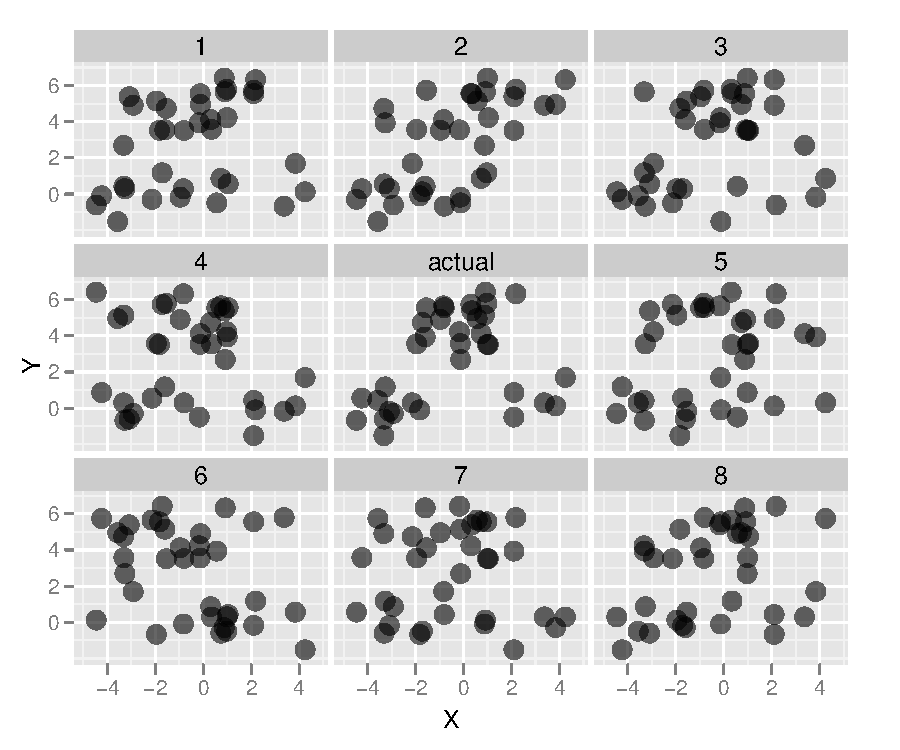
\includegraphics{minimum.pdf}}
	\vspace{-.2in}
       \caption{Lineup showing the actual plot and plots made of the permuted data which has the minimum distance from the actual plot according to the eight distance measures.  }
       \label{minimum}
\end{figure}      
%\newpage

\section{Datasets}

We do not want to restrict ourselves to any particular relationship between the two continuous variables $X$ and $Y$. The distance measure should be able to pick the effect of outliers and clusters in the data. So we come up with four different datasets which generalizes the relationship between $X$ and $Y$ as far as possible. \\

\subsection{DataSet 1}

%\normalsize

The first dataset deals with the linear relationship between $X$ and $Y$. \\

$X_i \sim \hbox{Normal}(0, 1)$ for $i = 1, 2, \dots, n.$ \\[0.2cm]
$Y_i = \beta_0 + \beta_1 x_i + \epsilon_i$ \\[0.3cm]
where $\beta_0 = 3.5$ and $\epsilon_i  \stackrel{iid}\sim \hbox{Normal}(0, \sigma)$. We take $\sigma = 6$. Such a dataset is presented in Figure \ref{data1}.\\
%where $\mu_X = 6$, $\sigma_X = 4$, $\beta_0 = 3.5$, $\beta_1 = 0.75$, $\sigma_Y = 6$.

\begin{figure}[hbtp]
%\begin{figurehere}
   \centering
       \scalebox{0.38}{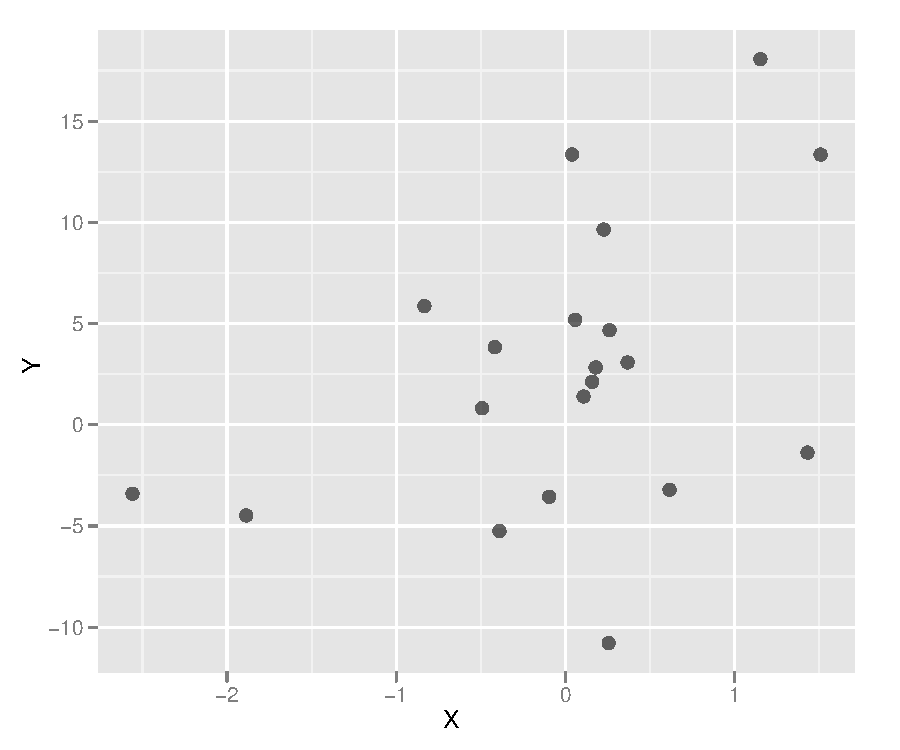
\includegraphics{data1.pdf}}
%      \scalebox{0.3}{\includegraphics{data1_30_5_1.pdf}}
%       \scalebox{0.3}{\includegraphics{data1_50_5_1.pdf}}
       \caption{One typical example of dataset 1.}
       \label{data1}
%	\vspace{-.1in}
\end{figure}

%\begin{figure}[hbtp]
%%\begin{figurehere}
%   \centering
%       \scalebox{0.3}{\includegraphics{data1_20_1_1.pdf}}
%       \scalebox{0.3}{\includegraphics{data1_20_3_1.pdf}}
%       \scalebox{0.3}{\includegraphics{data1_20_6_1.pdf}}
%       \caption{Different values of $\beta$ -- 0.1, 0.3 and 0.6 and $n = 20$.}
%	\vspace{-.1in}
%\end{figure}

%\subsection*{DataSet 2}

%\newpage

\subsection{DataSet 2}

%\normalsize

The second dataset is a dataset with contamination. To generate the contaminated data set of size $n = 50$ we used the following model

\[ X_i \sim \left\{ \begin{array}{ll}
         \hbox{Normal} (0, 1) & \mbox{for $i = 1,2, \dots, n_1$}\\
        \hbox{Normal} (\mu, 1/3) & \mbox{for $i = 1,  \dots, n_2$}.\end{array} \right. \]

\[ Y_i \sim \left\{ \begin{array}{ll}
         5 + \beta_1 X_i + \epsilon_i  & \mbox{for $i = 1,2, \dots, n_1$}\\
         20 + \eta_i & \mbox{for $i = 1, \dots, n_2$}.\end{array} \right. \]
         
where  $\epsilon_i \sim N(0, \sigma)$, $\eta_i \sim N(0, \sigma/3)$ , $\mu = -1.75$ and $n = n_1 + n_2$.  We use $\sigma = 5$, $n_1 = 40$ and $n_2 = 10$. \\      

\begin{figure}[hbtp]
%\begin{figurehere}
   \centering
       \scalebox{0.38}{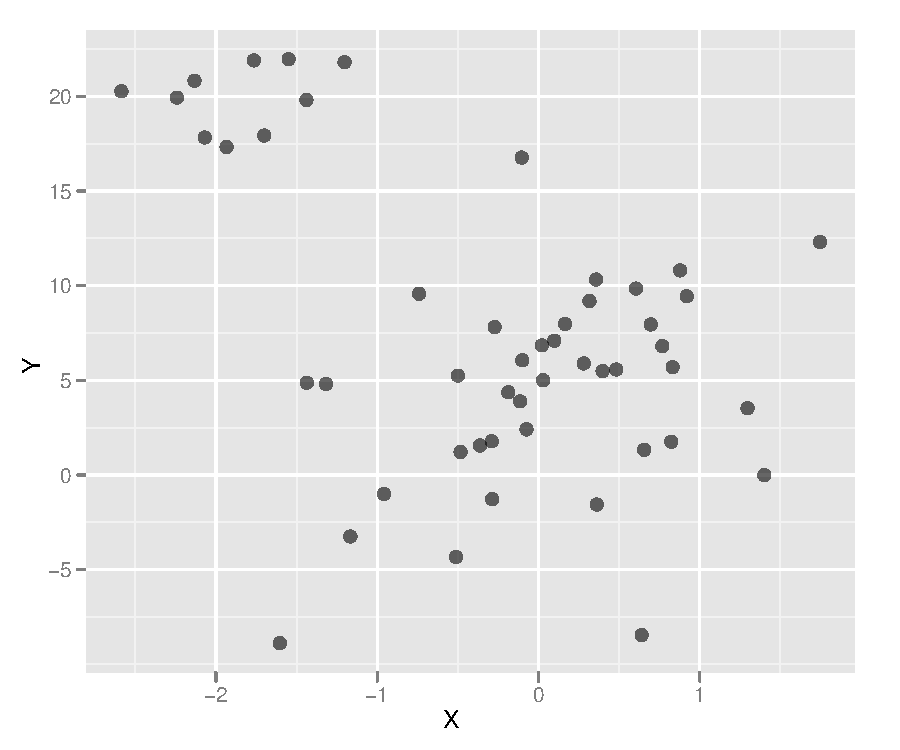
\includegraphics{data2.pdf}}
%      \scalebox{0.3}{\includegraphics{data1_30_5_1.pdf}}
%       \scalebox{0.3}{\includegraphics{data1_50_5_1.pdf}}
       \caption{One typical example of dataset 2.}
       \label{data2}
%	\vspace{-.1in}
\end{figure}
        
%        where $\mu_{X1} = 12$, $\mu_{X2} = 40$, $\sigma_{X1} = 6$, $\sigma_{X2} =  \sigma_{Y2} = 0.5$, $\beta_0 = 4.5$, $\beta_1 = 0.375$, $\sigma_{Y1} = 6$.
        
%\begin{figure}[hbtp]
%%\begin{figurehere}
%   \centering
%       \scalebox{0.4}{\includegraphics{data2_40_5_1.pdf}}
%       \scalebox{0.4}{\includegraphics{data2_40_08_1.pdf}}
%       \caption{Different values of $\beta$ (positive and negative)}
%	\vspace{-.1in}
%\end{figure}        
        
%\subsection*{DataSet 3}

%\newpage

\subsection{DataSet 3}

%\normalsize

The third dataset is a dataset where as $X$ increases, the variability in $Y$ increases first and then decreases.

\[ X_i \sim \left\{ \begin{array}{ll}
         \hbox{Normal} (15, 0.5) & \mbox{for $i = 1,2, \dots, n_1$}\\
        \hbox{Normal} (15, 3) & \mbox{for $i = 1,  \dots, n_2$}.\end{array} \right. \]

\[ Y_i \sim \left\{ \begin{array}{ll}
         \hbox{Normal} (40 , 8) & \mbox{for $i = 1,2, \dots, n_1$}\\
        \hbox{Normal}  (15 , 7) & \mbox{for $i = 1, \dots, n_2$}.\end{array} \right. \]
        
 where we take $n_1 = 5$, $n_2 = 35$ and $n = n_1 + n_2 = 40$. \\       
 
 \begin{figure}[hbtp]
%\begin{figurehere}
   \centering
       \scalebox{0.38}{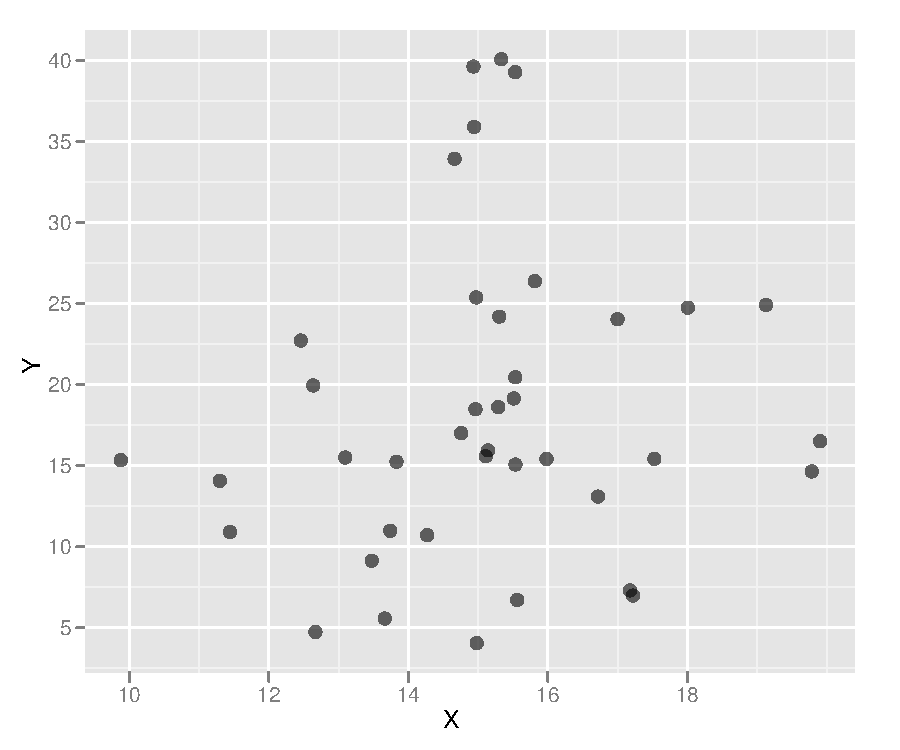
\includegraphics{data3.pdf}}
%      \scalebox{0.3}{\includegraphics{data1_30_5_1.pdf}}
%       \scalebox{0.3}{\includegraphics{data1_50_5_1.pdf}}
       \caption{One typical example of dataset 3.}
       \label{data3}
%	\vspace{-.1in}
\end{figure}

%\begin{figure}[hbtp]
%%\begin{figurehere}
%   \centering
%       \scalebox{0.4}{\includegraphics{data3_40_1.pdf}}
%       \caption{Dataset 3}
%	\vspace{-.1in}
%\end{figure}

%\subsection*{DataSet 4}

%\newpage

\subsection{DataSet 4}

%\normalsize

The fourth and final dataset has 3 visible clusters, which are 6 units apart from each other.\\ 

$\epsilon_i \stackrel{iid}\sim \hbox{Normal} (0, 1)$ for $i = 1, 2, \dots, n.$ \\[0.2cm]
$X_i  = \theta + \epsilon_i$ \\
$Y_i = \delta + \epsilon_i$ \\
where 

\[ (\theta, \delta) \sim \left\{ \begin{array}{ll}
         (-3, 0) & \mbox{for $\qquad i = 1,2, \dots, n_1$}\\
        	(3, 0) & \mbox{for  $\qquad i = n_1 + 1, \dots, n_1 + n_2$}\\
        	(0, \sqrt{27}) & \mbox{for  $\qquad i = n_1 + n_2 + 1, \dots, n$}\\
        \end{array} \right. \]
        
        
        where $n = n_1 + n_2 + n_3.$
        
 \begin{figure}[ht]
%\begin{figurehere}
   \centering
       \scalebox{0.35}{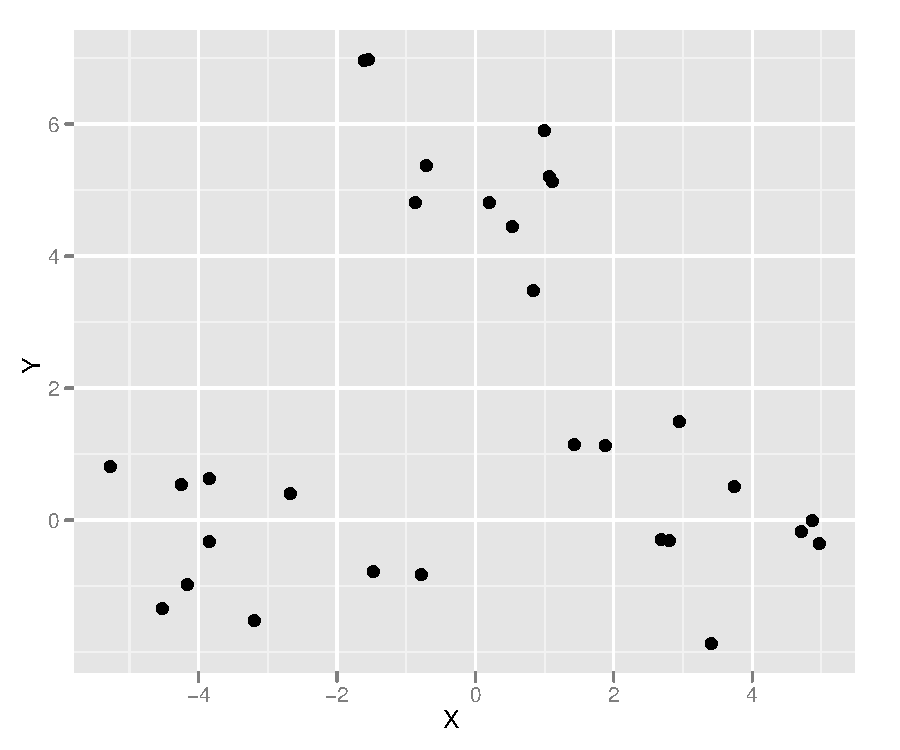
\includegraphics{data4.pdf}}
%      \scalebox{0.3}{\includegraphics{data1_30_5_1.pdf}}
%       \scalebox{0.3}{\includegraphics{data1_50_5_1.pdf}}
       \caption{One typical example of dataset 4.}
       \label{data4}
%	\vspace{-.1in}
\end{figure}   

\newpage

\section{Plans and Time Line}

\subsection{Jobs completed}

\begin{table}[hbtp]
\caption{Jobs completed so far}
\centering 
\begin{tabular}{|l|p{10cm}|r|} 
\hline
Task &  Description & Status date\\ %[0.5ex] % inserts table %heading 
\hline
Large p, small n & A comparison was done between data with real separation and data with no real separation to examine the performance of projection pursuit in \texttt{tourr} package \vspace{.1in} & Jan 2011 \\
Poster & Poster presented in the 4th Annual Midwest Statistics Research Colloquium\vspace{.1in} & Mar 2011 \\ 
Pilot Study & 1st pilot study to examine the performance of projection pursuit.  \vspace{.1in} & May 2011\\ 
%Turk Experiment & The first Amazon Mechanical Turk experiment for obtaining the power of visual inference described in chapter 2. Our web site is used to collect data from the participants recruited from Amazon Mechanical Turk \vspace{.1in} & Nov 2010 \\
Talk & Presented the results of Chapter 2 in Joint Statistical Meetings, Miami Florida \vspace{.1in} & July 2011 \\
Paper & The paper titled ``Where's Waldo: Looking closely at a Lineup" submitted to ASA and won student paper award 2012 \vspace{.1in} & Dec 2011 \\

Developments in Chapter 3 & A method introduced to find a distance measure which works best as a visual distance \vspace{.1in} & April 2012\\
\hline
\end{tabular}
\label{tbl:cjob}
\end{table}	

\subsection{Scheduled deliverables}

\begin{table}[hbtp]
\caption{Jobs to be completed}
\centering 
\begin{tabular}{|l|p{10cm}|r|} 
\hline
Task &  Description & Status date\\ %[0.5ex] % inserts table %heading 
\hline
Chapter 4 & I will develop the teaching materials in Chapter 4 during the summer. I have made some materials for my Stat 226 class for Spring 2011 and only 20\% work is complete\vspace{.1in} & July 2012 \\
Talk & Present the paper that won the ASA student paper award 2012 in JSM \vspace{.1in} & Aug 2012\\
Turk Experiment & The first turk experiment to examine which distance measure among a selected set works closest to the visual distance  \vspace{.1in}& Sep 2012 \\
Paper & The paper based on Large p, small n materials \vspace{.1in} & Oct 2012 \\
R Package  & Based on the results of the turk experiment, R package to provide measure of the quality of a lineup.  \vspace{.1in} & Nov 2012\\
Paper & The paper based on the analysis of turk data and Chapter 3 materials. \vspace{.1in} & Dec 2012\\
Work on Real dataset & Start working on analysis of Large Datasets using visual inference \vspace{.1in}  & Mar 2013\\ 
Thesis defense & Planned thesis defense \vspace{.1in} & May 2013\\
%Paper & Paper based on the real data analysis and implementation of visual inference technique with medical data from summer internship with Novartis \vspace{.1in} & May 2012\\
\hline 
\end{tabular}
\label{tbl:tjob}
\end{table}	

%\subsection{Other Works} This work may not contribute to this thesis.
%
%\subsubsection{Mathematical Framework of Visual Inference}
%In visual inferential procedure, the test statistic is a plot which is not a random variable in classical definition. But it is a function of data and hence inherits uncertainty due to sampling variations. Thus it is required to broaden the scope of the definition of random variable to bring the statistical inference world under a more general mathematical framework.
%
%Mathematicians have done a lot of work to give the mathematical framework for statistical methods and procedures. But statistical techniques are expanding its horizon and due to practical necessity it is not limiting its fundamental base on some limited mathematical framework. Visual statistical inference is such an example. This is where we need to focus on how we can come up with a more general mathematical framework for statistical inference as a whole. 
%
%As we see in chapter 2, the concept of the power of a visual test is no more depending on some limited regularity conditions. Rather, the fundamental classical assumption for uniformly most powerful (UMP) test made it more vulnerable in front of newly developed visual inference procedure. In this perspective we need to focus on making the current mathematical framework more general to incorporate broader area of inferential statistics. I intend to work on this area in near future.
%
%\subsubsection{Tool for Statistics Education} From our turk experiment we observed that significant number of evaluations are correct even though turker's education level is not even graduate. Even if the turkers are well educated they have no idea what the experiment is about. But still their evaluations indicates strong power of statistical inference. This suggests that Statistical Inference could be introduced to the students earlier than what we usually do now since it does not require a lot of technical knowledge. Visual Inference technique could be their first step in learning statistical inference. This would make a strong mindset about the core of statistical inference with less effort but with lot of fun. That would be another direction of research.  
